\documentclass{article}


\usepackage{arxiv}

\usepackage[utf8]{inputenc} % allow utf-8 input
\usepackage[T1]{fontenc}    % use 8-bit T1 fonts
\usepackage{hyperref}       % hyperlinks
\usepackage{url}            % simple URL typesetting
\usepackage{booktabs}       % professional-quality tables
\usepackage{amsfonts}       % blackboard math symbols
\usepackage{nicefrac}       % compact symbols for 1/2, etc.
\usepackage{microtype}      % microtypography
\usepackage{lipsum}
\usepackage{graphicx}
\usepackage[portuguese]{babel}
%\graphicspath{{figures/}{pdf/}}

\title{Modelo computacional do sistema neuromuscular} %A template for the \emph{arxiv} style}


\author{
  Heitor S.~Fernandes\\
  %David S.~Hippocampus\thanks{Use footnote for providing further
  %  information about author (webpage, alternative
  %  address)---\emph{not} for acknowledging funding agencies.} \\
  Departamento de Engenharia Biomédica\\
  Faculdade de Engenharia Elétrica e de Computação\\
  Universidade Estadual de Campinas\\
  \texttt{heitorsf@gmail.com} \\
  %% examples of more authors
  %% \AND
  %% Coauthor \\
  %% Affiliation \\
  %% Address \\
  %% \texttt{email} \\
  %% \And
  %% Coauthor \\
  %% Affiliation \\
  %% Address \\
  %% \texttt{email} \\
  %% \And
  %% Coauthor \\
  %% Affiliation \\
  %% Address \\
  %% \texttt{email} \\
}

\begin{document}
\maketitle

\begin{abstract}
%\lipsum[1]
Neste trabalho é apresentado um modelo computacional de um núcleo motor (composto por três motoneurônios alfa) e as respectivas unidades musculares. O modelo neuromuscular é constituído por unidades motoras dos tipos S, FR e FF, que foram implementadas computacionalmente utilizando a linguagem de programação Python e as bibliotecas do simulador NEURON. O modelo representou aspectos fundamentais do funcionamento do sistema neuromuscular como, por exemplo, a relação entre a força e a frequência de ativação das unidades motoras, bem como a ordem de recrutamento e a modulação da frequência de disparos de potenciais de ação das unidades motoras durante a geração da força muscular. Os códigos-fonte estão disponíveis em https://github.com/heitorsf/reproducible.
\end{abstract}


% keywords can be removed
\keywords{controle da força muscular \and modelagem computacional \and unidade motora}


\section{Introdução}
A simulação computacional de modelos matemáticos tem sido utilizada em neurociências e auxiliado o estudo e a compreensão de mecanismos envolvidos no funcionamento do sistema nervoso, que podem ser difíceis por meio exclusivo da experimentação. Especificamente, para o sistema neuromuscular humano, modelos matemáticos multiescala (que representam mecanismos operando em níveis celulares e/ou moleculares até elementos macroscópicos, como os processos de geração e controle da força muscular) têm possibilitado estudos sobre os comportamentos dinâmicos de redes de motoneurônios alfa (MNs) controlando a geração de força muscular [1-5]. Estes estudos fornecem subsídios conceituais para uma maior compreensão de aspectos neurofisiológicos do controle motor, como, por exemplo: i) os papéis do recrutamento e da modulação da frequência de disparos de potenciais de ação (PAs) na relação força-EMG [1]; ii) a atuação de vias de realimentação sensorial no controle da força muscular [2]; iii) o efeito de condições patológicas no controle reflexo da força [3]; e iv) o efeito de entradas neuromodulatórias na atividade de MNs individuais e na variabilidade da força muscular [4]. Além destas aplicações científicas importantes, modelos computacionais do sistema nervoso e muscular podem ser utilizados como ferramentas didáticas em cursos de Neurociências e Controle Motor [5].

O desenvolvimento de um modelo computacional envolve decisões relacionadas a dois aspectos principais: 1) o nível de complexidade do sistema físico ou biológico que o modelo matemático pretende representar e 2) a plataforma computacional na qual o modelo é implementado. O primeiro está associado, em algum grau, à plausibilidade biológica do modelo e à sua eficiência computacional, enquanto o segundo está relacionado ao uso de linguagens de programação livres, versáteis, de fácil aprendizado e utilização para os pesquisadores das diferentes áreas do conhecimento. Do ponto de vista do sistema neuromuscular, alguns dos modelos citados anteriormente [1-5], embora apresentem uma boa fidelidade biológica, foram desenvolvidos em plataformas proprietárias (e.g. Matlab) ou em linguagens que não são tipicamente utilizadas atualmente por pesquisadores na área de Neurociências, criando, portanto, barreiras adicionais à ampla utilização destes modelos.

Neste estudo, o objetivo é o desenvolvimento de um modelo multiescala simplificado do sistema neuromuscular. O modelo foi concebido de forma a possuir plausibilidade biológica e eficiência computacional. Além disso, para a implementação computacional dos modelos, foram adotadas plataformas flexíveis e reconhecidas pela comunidade científica da área de Neurociências.

%\section{Headings: first level}
\section{Métodos}
O modelo foi implementado em linguagem de programação Python (versão 2.7.13), que é uma linguagem livre, de fácil entendimento \cite{Lutz2013} e que vem sendo utilizada e difundida pela comunidade científica de Neurociência Computacional \cite{Muller2015}. Os elementos neuronais foram implementados utilizando as bibliotecas do simulador NEURON \cite{carnevale2006neuron} para a linguagem Python. A rede de MNs foi implementada utilizando o NetPyNE \cite{Dura-Bernal2016}.

O modelo neuromuscular desenvolvido é composto por apenas três MNs (modelo simplificado) e as fibras musculares por eles inervadas. As fibras musculares pertencentes a uma determinada unidade motora são referidas como unidades musculares (UMs). Os modelos individuais dos MNs e das UMs serão descritos abaixo.

\paragraph{Modelo de MN alpha}
Foram representados modelos de MNs dos tipos S (\emph{slow}, que inerva fibras musculares lentas e resistentes à fadiga), FR (\emph{fast fatigue resistant}, fibras rápidas e resistentes à fadiga) e FF (\emph{fast fatigable}, fibras rápidas e fatigáveis). Estes modelos foram baseados na proposta de Cisi e Kohn \cite{Cisi2008a}, em que a morfologia dos MNs é sintetizada em dois compartimentos acoplados por uma condutância. Um compartimento representa a árvore dendrítica, que neste estudo foi suposta passiva, e o outro compartimento representa o corpo celular (ou soma). O circuito elétrico equivalente dos modelos está ilustrado na Figura 1. As condutâncias ativas somáticas são responsáveis pelo decurso temporal do PA e da AHP (\emph{after hyperpolarization}). Estas condutâncias (Na+, K+, persistente de Na+ e lenta de K+) foram parametrizadas e validadas em um estudo anterior do nosso laboratório \cite{Matoso2017}, sendo que os parâmetros geométricos e eletrotônicos (Tabela 1) foram baseados em estudos experimentais anteriores com MNs de gatos anestesiados \cite{Crill1996,Fleshman1988,Zengel1985}.

\begin{figure}[h]
  \centering
  \fbox{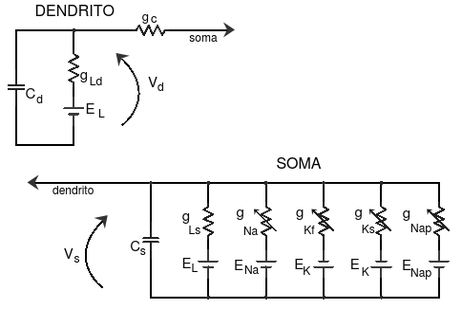
\includegraphics[width=7cm]{../figures/pdf/Circuito}}
  \caption{Circuito elétrico equivalente representando o soma e o dendrito dos modelos de MNs. $E_Na$ e $E_K$ representam os potenciais de equilíbrio dos íons Na+ e K+, respectivamente. $E_L$ representa o potencial de repouso da membrana. As condutâncias $g_Ld$, $g_Ls$, $g_c$, $g_Na$,$g_Kf$, $g_Ks$, $g_Nap$, representam as condutâncias de fuga dendrítica e somática, de acoplamento, de Na+, rápida de K+, lenta de K+ e persistente de Na+, respectivamente. $C_d$ e $C_s$ representam as capacitâncias de membrana dendrítica e somática.}
  \label{fig:fig1}
\end{figure}

Para o axônio, adotou-se um modelo simplificado baseado na detecção de um PA e sua transmissão até a UM com uma dada velocidade de condução. Os valores de velocidade de condução axonal foram baseados em estudos anteriores \cite{Cisi2008a} (Tabela 2). O limiar de detecção do PA foi definido como o instante em que a taxa de variação do potencial de membrana é igual (ou ligeiramente superior) a 10mV/ms \cite{Elias2012}. Adotou-se uma distância de 0,60 m entre o MN e a UM.

\paragraph{Modelo de Unidade Muscular}
As UMs foram modeladas como a resposta ao impulso (em tempo discreto) de um sistema de segunda ordem criticamente amortecido. Neste sistema são definidos dois parâmetros: i) a amplitude máxima do abalo muscular e ii) o tempo de contração (intervalo entre o início do abalo e o instante em que se atinge a amplitude máxima). Além disso, adotou-se um mecanismo forçado de saturação (baseado na frequência de disparos de PAs do MN) para as forças tetânicas das UMs. Os parâmetros dos modelos das UMs dos tipos S, FR e FF encontram-se na Tabela 2 e foram baseados em dados experimentais do tríceps sural humano \cite{Watanabe2013}.

\begin{table}[h]
 \caption{Parâmetros dos modelos de MN.}
  \centering
  \begin{tabularx}{\columnwidth}{Xlll}
    \toprule
   % \multicolumn{2}{c}{Part}                   \\
    %\cmidrule(r){1-2}
    Parâmetro     & Tipo S     & Tipo FR     & Tipo FF   \\
    \midrule
    Capacitância específica [F/cm2] & 1 & 1 & 1    \\
    Resistividade citoplasmática [Ohm-cm2] & 70 & 70 & 70 \\
    Comprimento (dendrito) [mm] & 6,15 & 7,45 & 9,35 \\
    Diâmetro (dendrito) [um] & 52 & 73 & 88 \\
    Resistência específica (dendrito) [kOhm-cm2] & 12,55 & 8,83 & 6,50 \\
    Comprimento (soma) [um] & 80 & 85 & 100,25 \\
    Diâmetro (soma) [um] & 80 & 85 & 100,25 \\
    Resistência epecífica (soma) [kOhm-cm2] & 1,10 & 1,0 & 0,80 \\
    Velocidade de condução axonal [m/s] & 45,5 & 48,5 & 51,5 \\
   % Axon     & Output terminal & $\sim$10      \\
    %Soma     & Cell body       & up to $10^6$  \\
    \bottomrule
  \end{tabularx}
  \label{tab:table1}
\end{table}

% Size ($\mu$m);   $\sim$100

\begin{table}[h]
 \caption{Parâmetros das unidades musculares.}
  \centering
  \begin{tabular}{llll}
    \toprule
   % \multicolumn{2}{c}{Part}                   \\
    %\cmidrule(r){1-2}
    Parâmetro     & Tipo S     & Tipo FR     & Tipo FF   \\
    \midrule
    Amplitude do abalo [N] & 1,70 & 1,90 & 2,15 \\
    Tempo de contração [ms] & 110,0 & 73,5 & 55,0 \\
    Frequência de saturação [Hz] & 20 & 40 & 60 \\
    \bottomrule
  \end{tabular}
  \label{tab:table2}
\end{table}

\paragraph{Protocolo de Simulação: Relação força-frequência das unidades motoras}
Todas as simulações foram realizadas utilizando-se o método numérico de integração de Euler com passo fixo de 1 ms. Foram realizados dois protocolos experimentais que serão descritos a seguir. Foram feitas simulações para verificar a relação entrada-saída de cada unidade motora. Para tanto, cada MN do núcleo motor foi estimulado com degraus de corrente com diferentes intensidades, de forma a promover disparos repetitivos de PAs com diferentes frequências. Em cada condição, registrou-se a força gerada pelas unidades motoras a fim de se obter a relação entre a força da UM e a frequência de ativação do MN \cite{Kernell2006}.

\paragraph{Protocolo de simulação: Princípio do tamanho e geração da força muscular}
Neste protocolo, buscou-se verificar a capacidade do modelo em representar as duas estratégias principais do sistema neuromuscular no controle de força: o recrutamento de unidades motoras (recruitment coding) e a modulação de suas frequências de disparos de PA (rate coding) \cite{kandel2013}. O núcleo motor foi estimulado por uma corrente com forma de onda triangular simétrica (pico de 22 nA) e duração de 5 segundos. A força total gerada pelo modelo simplificado de músculo foi definida como a soma das forças geradas pelas UMs.
%\label{sec:headings}

%\lipsum[4] See Section \ref{sec:headings}.

\section{Resultados}
\paragraph{Relação força-frequência das unidades motoras}
Na Figura 2 observa-se que a relação força-frequência apresenta uma região linear para os três tipos de unidades motoras; porém, a força tetânica de cada unidade motora é diferente, sendo que as unidades motoras dos tipos S, FR e FF apresentaram forças tetânicas máximas de aproximadamente 10 N, 15 N e 19 N, respectivamente. Uma maneira de avaliar a propriedade contrátil da UM é medindo-se a relação entre a amplitude máxima do abalo muscular e a força tetânica máxima (relação twitch/tétano) [15]. Nos modelos das unidades motoras dos tipos S, FR e FF estes valores foram de 16,8\%, 18,6\% e 11,1\%, respectivamente.

%FIGURA

\paragraph{Princípio do tamanho e geração da força muscular}
Na parte inferior da Figura 3 estão indicados os instantes de disparos dos MNs de cada tipo (S em azul, FR em verde e FF em magenta). Os pontos na parte superior da Figura 3 indicam as frequências instantâneas de disparo dos MNs (mesmo código de cores) e a linha preta contínua representa a força total exercida pelo modelo simplificado de músculo. Nota-se que a unidade motora do tipo S é a primeira a ser recrutada, pois seu MN possui uma menor área celular (vide Tabela 1) e, consequentemente, uma maior resistência de entrada. Por outro lado, a unidade motora do tipo FF é a última a ser recrutada, pois o MN possui uma maior área celular e menor resistência de entrada. Além disso, observa-se nos resultados a ordem inversa de derrecrutamento, com a unidade motora de maior limiar (tipo FF) sendo derrecrutada primeiro e a de menor limiar (tipo S) por último.

\begin{figure}[h]
  \centering
  \fbox{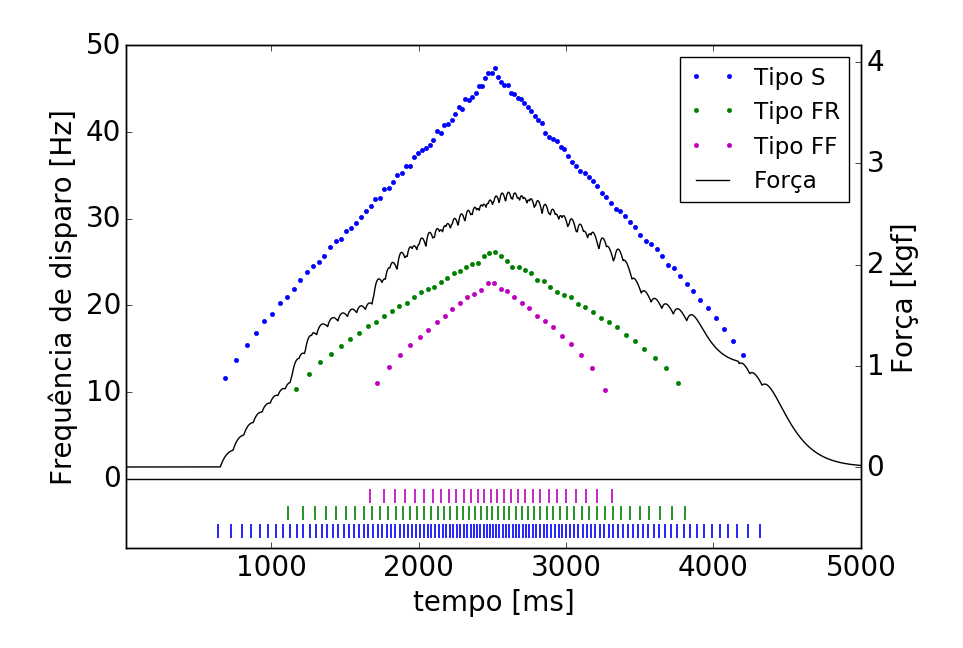
\includegraphics[width=7cm]{../figures/pdf/OnionSkin}}
  \caption{Mecanismos de controle e geração da força muscular. Os pontos coloridos representam as frequências de disparos dos MNs dos tipos S, FR e FF;os traços coloridos abaixo indicam os instantes de disparos dos PAs dos MNs; e a curva preta mostra avariação da força ao longo do tempo.}
  \label{fig:fig3}
\end{figure}

Do ponto de vista das frequências de disparos de PAs, observa-se que as unidades motoras recrutadas com um menor limiar atingem taxas de disparos maiores em comparação com as unidades motoras de maior limiar, para uma mesma magnitude da corrente de estimulação.

Quanto à geração da força muscular, nota-se na Figura 3 (linha preta) que a unidade motora do tipo S gera uma força relativamente pequena, mesmo com o aumento da sua frequência de disparos (pontos azuis) devido à menor amplitude dos abalos musculares e à força tetânica. À medida que novas unidades motoras são recrutadas (dos tipos FR e FF) a força aumenta, tanto pelo fato de estas unidades motoras produzirem abalos de maior magnitude, quanto por aumentarem as suas frequências de disparos (devido ao aumento da despolarização da membrana dos MNs pela corrente triangular). Observa-se, ainda, que quando as unidades motoras de maior limiar são recrutadas há um aumento na flutuação da força, pois os abalos não fundidos destas unidades motoras são mais evidentes.

%FIGURA

\section{Discussão}
Neste trabalho, foi desenvolvido um modelo multiescala do sistema neuromuscular humano contendo modelos de MNs e UMs biologicamente plausíveis e computacionalmente eficientes. Para a implementação do modelo foram utilizadas a linguagem de programação Python e o simulador NEURON [8]. Estas plataformas computacionais são flexíveis e reconhecidas pela comunidade científica da área de Neurociência, o que possibilitará uma ampla utilização deste modelo em estudos sobre o controle neurofisiológico da força muscular.

Pelas simulações realizadas neste estudo, pôde-se perceber que o modelo apresenta as propriedades básicas do sistema neuromuscular. Por exemplo, embora a saturação da força de uma dada UM tenha sido implementada de maneira relativamente simples, as relações força-frequência e as relações twitch/tétano são similares aos dados reportados na literatura experimental [15].

Outros aspectos representados de forma satisfatória pelo modelo são os mecanismos de controle da força muscular (Figura 3). O fato de os modelos de MNs terem uma representação biologicamente plausível e terem sido parametrizados de acordo com o princípio do tamanho [17] faz com que o recrutamento das unidades motoras e a modulação da frequência de disparos de PAs sejam compatíveis com as observações experimentais durante o controle da força isométrica em músculos esqueléticos. Além disso, a ordem de recrutamento e modulação em frequência, em que a primeira unidade motora a ser recrutada atinge frequências mais elevadas e é a última a ser derrecrutada, produz um fenômeno que é conhecido na literatura como onion skin, que parece ser um mecanismo intrínseco ao sistema neuromuscular para o controle da força [18].

\section{Conclusão}
O modelo do sistema neuromuscular proposto neste estudo representa as características básicas do sistema neuromuscular para o controle e a geração da força muscular. Desenvolvimentos posteriores, utilizando como base este modelo neuromuscular, terão como foco a modelagem de núcleos motores com um maior número de MNs, bem como UMs parametrizadas com base em dados de músculos esqueléticos de seres humanos. Desta forma, será possível comparar os resultados dos modelos com dados experimentais e explorar conceitualmente como mecanismos neurofisiológicos podem ser associados ao controle da força de um dado músculo.

\bibliographystyle{unsrt}  
%\bibliography{references}  %%% Remove comment to use the external .bib file (using bibtex).
%%% and comment out the ``thebibliography'' section.


%%% Comment out this section when you \bibliography{references} is enabled.
\begin{thebibliography}{1}

\bibitem{kour2014real}
George Kour and Raid Saabne.
\newblock Real-time segmentation of on-line handwritten arabic script.
\newblock In {\em Frontiers in Handwriting Recognition (ICFHR), 2014 14th
  International Conference on}, pages 417--422. IEEE, 2014.

\bibitem{kour2014fast}
George Kour and Raid Saabne.
\newblock Fast classification of handwritten on-line arabic characters.
\newblock In {\em Soft Computing and Pattern Recognition (SoCPaR), 2014 6th
  International Conference of}, pages 312--318. IEEE, 2014.

\bibitem{hadash2018estimate}
Guy Hadash, Einat Kermany, Boaz Carmeli, Ofer Lavi, George Kour, and Alon
  Jacovi.
\newblock Estimate and replace: A novel approach to integrating deep neural
  networks with existing applications.
\newblock {\em arXiv preprint arXiv:1804.09028}, 2018.

\end{thebibliography}

\end{document}